% !TeX root = 数字电路.tex
% ============================================================
%  封面：李思风（极简学术）—— 白底、居中标题、无装饰边框
%  参照《线性代数：原理与应用》（李思，清华大学）封面版式
%
%  可用字段（在主文件导言区 \newcommand 预定义即可覆盖）：
%    \notename      主标题（必填，主文件定义）
%    \noteauthor    作者（必填，主文件定义）
%    \notesubtitle  标题下方小字，默认 \today（日期/版本行）
%    \noteextra     底部单位/学院行，默认不显示
%
%  说明：中部线稿为可删装饰（半加器：异或门求和、与门进位），整段
%        \begin{tikzpicture}...\end{tikzpicture} 删除后即为纯文字极简封面。
%
%  版面做法：全页各段间距用「按原比例加权的 fil 弹性空白」而不是固定 \vspace，
%        整块装进 \vbox to \textheight，因此本页永远恰好占满版心：
%        既不会像固定间距那样把底部单位行挤到下一页，也能随字号、插图高度自动分配。
%        权重 4.7 / 4.1 / 3.4 / 4.3 / 1.8 / 1.6 即原来的 cm 间距比例。
% ============================================================
\begin{titlepage}
	\thispagestyle{empty}
	\providecommand{\notesubtitle}{\today}
	\providecommand{\noteextra}{}
	\centering
	\vbox to \textheight{%
		\vskip 0pt plus 4.7fil

		% ---- 主标题 ----
		{\bfseries\songti\fontsize{24.8}{30}\selectfont \notename\par}
		\vskip 0pt plus 4.1fil

		% ---- 日期 / 版本行 ----
		{\songti\fontsize{14.4}{18}\selectfont （\notesubtitle）\par}
		\vskip 0pt plus 3.4fil

		% ---- 手绘风极简线稿：半加器（异或门求和、与门进位，可整段删除）----
		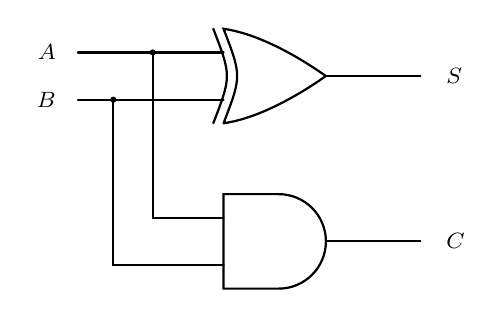
\begin{tikzpicture}[line width=0.8pt, line cap=round]
			% 输入 A、B 及其分支（A 的分支跨过 B 的输入线，为不连接的交叉）
			\draw (-2.40,1.45) -- (-0.55,1.45);
			\draw (-2.40,0.85) -- (-0.55,0.85);
			\fill (-1.45,1.45) circle (1.1pt);
			\draw (-1.45,1.45) -- (-1.45,-0.65) -- (-0.55,-0.65);
			\fill (-1.95,0.85) circle (1.1pt);
			\draw (-1.95,0.85) -- (-1.95,-1.25) -- (-0.55,-1.25);

			% 异或门：弧形后背 + 一条平行短弧
			\draw (-0.55,0.55)
				.. controls (-0.20,0.60) and (0.25,0.80) .. (0.75,1.15)
				.. controls (0.25,1.50) and (-0.20,1.70) .. (-0.55,1.75)
				.. controls (-0.32,1.15) .. (-0.55,0.55);
			\draw (-0.68,0.55) .. controls (-0.45,1.15) .. (-0.68,1.75);

			% 与门：直边 + 半圆
			\draw (-0.55,-1.55) -- (-0.55,-0.35) -- (0.15,-0.35)
				arc[start angle=90, end angle=-90, radius=0.60] -- cycle;

			% 输出：和 S、进位 C
			\draw (0.75,1.15) -- (1.95,1.15);
			\draw (0.75,-0.95) -- (1.95,-0.95);

			% 端口标注
			\node[font=\footnotesize, anchor=east] at (-2.55,1.45) {$A$};
			\node[font=\footnotesize, anchor=east] at (-2.55,0.85) {$B$};
			\node[font=\footnotesize, anchor=west] at (2.15,1.15) {$S$};
			\node[font=\footnotesize, anchor=west] at (2.15,-0.95) {$C$};
		\end{tikzpicture}\par
		\vskip 0pt plus 4.3fil

		% ---- 作者（楷体）----
		{\kaishu\fontsize{24.8}{30}\selectfont \noteauthor\par}
		\vskip 0pt plus 1.8fil

		% ---- 单位 / 学院（未定义则不显示）----
		{\songti\fontsize{20.7}{26}\selectfont \noteextra\par}
		\vskip 0pt plus 1.6fil
	}%
\end{titlepage}
